% id: 98-05
% book: 베이직쎈 확률과 통계 · 05 확률변수와 확률분포
% section: 실전 감각 UP
% figure: tikz:fig-98-05
% answer: 
% answer_source: 
% variant_level: 0 (원본 전사)
% 이 파일은 build.mjs 가 items.json 에서 만든다. 고칠 때는 items.json 을 고친다.
\smash{\raisebox{1.5mm}{\dmkichul{베이직쎈 확률과 통계 98쪽 05번 · 꼭 나와요}}}
$0\le x\le 3$에서 정의된 연속확률변수 $X$의 확률밀도함수 $f(x)$의 그래프가 다음 그림과 같을 때, $\mathrm{P}(0\le X\le 1)$은? \dmcondfill{$k$는 상수이다.}{}
\par\smallskip\begin{center}\resizebox{\ifdim\width>\linewidth\linewidth\else\width\fi}{!}{% 98-05(인쇄 98쪽) — 연속확률변수 X 의 확률밀도함수 y=f(x) 의 그래프(0 에서 k, 1 에서 3k 로 올랐다가 3 에서 0 으로 내려오는 꺾은선).
% 스캔 그래프가 흐려 TikZ 로 다시 그림. 라벨(3k · k · O · 1 · 3 · y=f(x))과 점선은 원문에 있는 것 그대로이고, 구하는 확률은 적지 않는다.
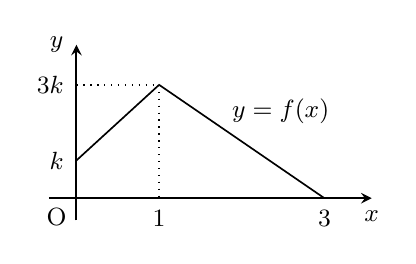
\begin{tikzpicture}[line width=0.5pt, font=\small]
  \draw[->, >=stealth, line width=0.7pt] (-0.35,0) -- (3.75,0) node[below=1pt] {$x$};
  \draw[->, >=stealth, line width=0.7pt] (0,-0.28) -- (0,1.95) node[left=1pt] {$y$};
  \node[below left=0pt] at (0,0) {O};
  \draw[line width=0.6pt] (0,0.48) -- (1.05,1.44) -- (3.15,0);
  \draw[dotted, line width=0.5pt] (0,1.44) -- (1.05,1.44);
  \draw[dotted, line width=0.5pt] (1.05,1.44) -- (1.05,0);
  \node[left=1pt] at (0,1.44) {$3k$};
  \node[left=1pt] at (0,0.48) {$k$};
  \node[below=1pt] at (1.05,0) {$1$};
  \node[below=1pt] at (3.15,0) {$3$};
  \node[above right=0pt] at (1.85,0.82) {$y=f(x)$};
\end{tikzpicture}
}\end{center}
\dmchoicesauto{\rule[-3ex]{0pt}{8ex}}{$\dfrac{2}{15}$}{$\dfrac{4}{15}$}{$\dfrac{2}{5}$}{$\dfrac{8}{15}$}{$\dfrac{2}{3}$}
